\chapter{Image Geometry}

\section{Linear 2D Transforms}

\subsection{Homogeneous 2D Point Coordinate}

\subsubsection{Basic Notational Conventions}

\begin{listu}
    \item Column-Vector Representation \[
        \begin{bmatrix}
            x \\
            y 
        \end{bmatrix}
    \]

    \item Row-Vector Representation \[
        \begin{bmatrix}
            x & y
        \end{bmatrix}
    \]

    \item Matrix Transpose Operation \[
        \begin{bmatrix}
            x \\
            y
        \end{bmatrix}^\top = \begin{bmatrix}
            x & y
        \end{bmatrix}
    \]
\end{listu}

\subsubsection{Homogeneous Coordinates}

In the standard Euclidean coordinate system, a point is represented by a pair of coordinates $(x, y)$, where $x$ and $y$ are the coordinates of the point along the $x$ and $y$ axes, respectively. 

\begin{center}
    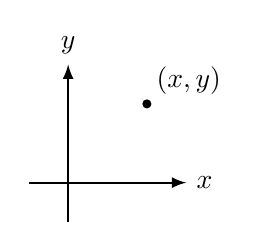
\begin{tikzpicture}[scale=0.5]
        \draw[thick,>=latex,->] (-1, 0) -- (3, 0) node[right] {$x$};
        \draw[thick,>=latex,->] (0, -1) -- (0, 3) node[above] {$y$};
        \draw[fill=black] (2, 2) circle (0.1) node[above right] {$(x, y)$};
    \end{tikzpicture}
\end{center}

In homogeneous coordinates, a point is represented by a triple of coordinates $(x, y, w)$, where $x$ and $y$ are the coordinates of the point along the $x$ and $y$ axes, respectively, and $w$ is a scaling factor that is normally set to $1$. The homogeneous coordinates of a point are not unique, since any multiple of the coordinates $(x, y, w)$ represents the same point. For example, $(2, 3, 1)$ and $(4, 6, 2)$ represent the same point. The homogeneous coordinates of a point are unique only up to a scaling factor. 

\begin{remark}
    Two vector of homogeneous coordinates $(x, y, w)$ and $(x', y', w')$ represent the same point if and only if there exists a non-zero scalar $\lambda$ such that \[
        \begin{bmatrix}
            x \\
            y \\
            w
        \end{bmatrix} = \lambda \begin{bmatrix}
            x' \\
            y' \\
            w'
        \end{bmatrix}
    \]
\end{remark}

\begin{example}
    The homogeneous coordinates of the point $(2, 3)$ are $(2, 3, 1)$, $(4, 6, 2)$, $(6, 9, 3)$, etc.
\end{example}

\subsubsection{Homogeneous to Euclidean Coordinat}

To convert a homogeneous coordinate $(x, y, w)$ to a Euclidean coordinate $(x', y')$, we divide the first two coordinates of the homogeneous coordinate by the third coordinate, i.e. \[
    \begin{bmatrix}
        x' \\
        y'
    \end{bmatrix} = \begin{bmatrix}
        x / w \\
        y / w
    \end{bmatrix}
\]

\begin{example}
    Plot the following points in the Euclidean plane: \[
        \begin{matrix}[l l l]
            P_1 = (2, 2, 2) & P_2 = (10, 0, 2) & P_3 = (0, 8, 4) \\
            P_4 = (1, 0, 0.01) & P_5 = (1, 0, 0) & P_6 = (0, 1, 0) \\
            P_7 = (1, 1, 0) & &
        \end{matrix}
    \]

    \begin{center}
        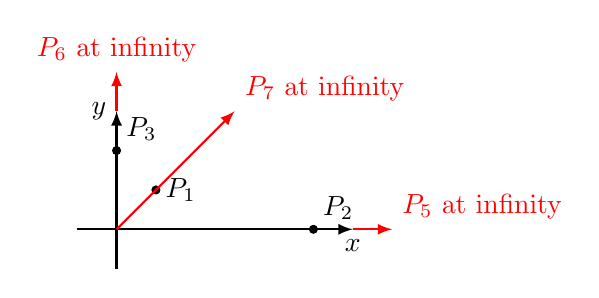
\begin{tikzpicture}[scale=0.5]
            \draw[thick,>=latex,->] (-1, 0) -- (6, 0) node[below] {$x$};
            \draw[thick,>=latex,->] (0, -1) -- (0, 3) node[left] {$y$};

            \draw[fill=black] (1, 1) circle (0.1) node[right] {$P_1$};
            \draw[fill=black] (5, 0) circle (0.1) node[above right] {$P_2$};
            \draw[fill=black] (0, 2) circle (0.1) node[above right] {$P_3$};

            \draw[thick,>=latex,->,red] (6, 0) -- (7, 0) node[above right] {$P_5$ at infinity};
            \draw[thick,>=latex,->,red] (0, 3) -- (0, 4) node[above] {$P_6$ at infinity};
            % P7
            \draw[thick,>=latex,->,red] (0, 0) -- (3, 3) node[above right] {$P_7$ at infinity};
        \end{tikzpicture}
    \end{center}

    Note that $P_5$, $P_6$, and $P_7$ are at infinity. This is a very important property of homogeneous coordinates. 
\end{example}

\begin{remark}
    Points infinitely far away from the origin in the Euclidean plane have a finite representation in homogeneous coordinates (i.e. $(x, y, 0)$). These points are sometimes called \term{ideal points}.
\end{remark}

\subsection{Homogeneous 2D Line Coordinates}

\subsubsection{Homogeneous 2D Line Coordinates}

\begin{remark}
    The general equation of a line in the Euclidean plane is \[
        ax + by + c = 0
    \] where $a$, $b$, and $c$ are real numbers and $a$ and $b$ are not both zero.

    In homogeneous coordinates, using the matrix notation, the general equation of a line is \[
        \begin{bmatrix}
            a & b & c
        \end{bmatrix} \begin{bmatrix}
            x \\ y \\ w
        \end{bmatrix} = 0
    \]
    Or, equivalently, \[
        \ell^\top p = 0
    \] where $\ell$ is the vector holding line coefficients and $p$ is the vector holding point coordinates.
\end{remark}

\begin{definition}
    The \term{homogeneous coordinates of a line} with the equation \[ ax + by + c = 0 \] is the vector \[ \ell = \begin{bmatrix} a \\ b \\ c \end{bmatrix} \]
\end{definition}

\begin{example}
    The homogeneous coordinates of the line $y = x$ is \[
        \ell = \begin{bmatrix}
            -1 \\ 1 \\ 0
        \end{bmatrix}
    \]
\end{example}

\subsubsection{Line Passing Through Two Points}

In this case, $\ell$ must satisfy the following equations: \[
    \ell^\top P_1 = 0 \qquad \ell^\top P_2 = 0
\] where $p_1$ and $p_2$ are the homogeneous coordinates of the two points.

We can take the cross product of $p_1$ and $p_2$ to obtain $\ell$: \[
    \ell = P_1 \times P_2
\]

\begin{remark}
    To compute the cross product of two vectors, we can use the following two methods. 

    \[
        \ell = \begin{bmatrix}
            x_1 \\ y_1 \\ z_1
        \end{bmatrix} \times \begin{bmatrix}
            x_2 \\ y_2 \\ z_2
        \end{bmatrix}
    \]

    {~~~}

    \begin{minipage}[t]{0.45\linewidth}
        As matrix multiplication: \[
            P_1 \times P_2 = \begin{bmatrix}
                0 & -z_1 & y_1 \\
                z_1 & 0 & -x_1 \\
                -y_1 & x_1 & 0
            \end{bmatrix} P_2
        \]
    \end{minipage}%
    \hfil%
    \begin{minipage}[t]{0.45\linewidth}
        As determinant: \[
            P_1 \times P_2 = \left| 
                \begin{matrix}
                    \color{red} i & \color{red} j & \color{red} k \\
                    x_1 & y_1 & z_1 \\
                    x_2 & y_2 & z_2
                \end{matrix}
            \right|
        \]
    \end{minipage}
\end{remark}

\subsubsection{Intersection of Two Lines}

In this case, $p$ must satisfy the following equations: \[
    \ell_1^\top p = 0 \qquad \ell_2^\top p = 0
\] where $\ell_1$ and $\ell_2$ are the homogeneous coordinates of the two lines.

We can take the cross product of $\ell_1$ and $\ell_2$ to obtain $p$: \[
    p = \ell_1 \times \ell_2
\]

\begin{remark}
    For parallel lines, we cannot compute its standard Euclidean intersection point. Instead, we can compute the homogeneous intersection point, which will be at infinity.
\end{remark}

\subsection{Affine 2D Transformations}

\begin{listu}
    \item \textbf{Identity} \[
        \begin{bmatrix}
            x' \\ y' \\ w'
        \end{bmatrix} \cong \begin{bmatrix}
            x \\ y \\ 1
        \end{bmatrix} = \begin{bmatrix}
            1 & 0 & 0 \\
            0 & 1 & 0 \\
            0 & 0 & 1
        \end{bmatrix} \begin{bmatrix}
            x \\ y \\ 1
        \end{bmatrix}
    \]

    \item \textbf{Stretching} (along $x$) \[
        \begin{bmatrix}
            x' \\ y' \\ w'
        \end{bmatrix} \cong \begin{bmatrix}
            {\color{red} s} x \\ y \\ 1
        \end{bmatrix} = \begin{bmatrix}
            1 & 0 & {\color{red} t} \\
            0 & 1 & 0 \\
            0 & 0 & 1
        \end{bmatrix} \begin{bmatrix}
            x \\ y \\ 1
        \end{bmatrix}
    \]
    
    \textbf{Stretching} (along $y$) \[
        \begin{bmatrix}
            x' \\ y' \\ w'
        \end{bmatrix} \cong \begin{bmatrix}
            x \\ {\color{red} s} y \\ 1
        \end{bmatrix} = \begin{bmatrix}
            1 & 0 & 0 \\
            0 & {\color{red} s} & 0 \\
            0 & 0 & 1
        \end{bmatrix} \begin{bmatrix}
            x \\ y \\ 1
        \end{bmatrix}
    \]

    \item \textbf{Shearing} (along $y$) \[
        \begin{bmatrix}
            x' \\ y' \\ w'
        \end{bmatrix} \cong \begin{bmatrix}
            x \\ {\color{red} h} x + y \\ 1
        \end{bmatrix} = \begin{bmatrix}
            1 & 0 & 0 \\
            {\color{red} h} & 1 & 0 \\
            0 & 0 & 1
        \end{bmatrix} \begin{bmatrix}
            x \\ y \\ 1
        \end{bmatrix}
    \]

    \item \textbf{Rotation} (about the origin bt angle $\phi$) \[
        \begin{bmatrix}
            x' \\ y' \\ w'
        \end{bmatrix} \cong \begin{bmatrix}
            {\color{red}(\cos \phi)} x {\color{red}- (\sin \phi)} y \\
            {\color{red}(\sin \phi)} x + {\color{red}(\cos \phi)} y \\
            1
        \end{bmatrix} = \begin{bmatrix}
            {\color{red}\cos \theta} & {\color{red}-\sin \theta} & 0 \\
            {\color{red}\sin \theta} & {\color{red}\cos \theta} & 0 \\
            0 & 0 & 1
        \end{bmatrix} \begin{bmatrix}
            x \\ y \\ 1
        \end{bmatrix}
    \]

    \item \textbf{Translation} (along $x$) \[
        \begin{bmatrix}
            x' \\ y' \\ w'
        \end{bmatrix} \cong \begin{bmatrix}
            x + {\color{red} d} \\ y \\ 1
        \end{bmatrix} = \begin{bmatrix}
            1 & 0 & {\color{red} d} \\
            0 & 1 & 0 \\
            0 & 0 & 1
        \end{bmatrix} \begin{bmatrix}
            x \\ y \\ 1
        \end{bmatrix}
    \]

    \textbf{Translation} (along $y$) \[
        \begin{bmatrix}
            x' \\ y' \\ w'
        \end{bmatrix} \cong \begin{bmatrix}
            x \\ y + {\color{red} d} \\ 1
        \end{bmatrix} = \begin{bmatrix}
            1 & 0 & 0 \\
            0 & 1 & {\color{red} d} \\
            0 & 0 & 1
        \end{bmatrix} \begin{bmatrix}
            x \\ y \\ 1
        \end{bmatrix}
    \]
\end{listu}

We can combine these transformations to form more complex transformations. For example, we can combine a rotation and a translation to form a \term{rotation about a point} transformation. 

\begin{definition}[Affine Transformation (Intuitive)]
    An \term{affine transformation} is any combination of scaling, shearing, rotation, and translation.

    \[ 
        \begin{bmatrix}
            a & b & c \\
            d & e & f \\
            0 & 0 & g
        \end{bmatrix} 
    \] where $g \neq 0$ is a scaling factor that does not affect the transformation.
\end{definition}

\begin{remark}
    An affine transformation is a transformation that preserves parallelism and ratios of distances along parallel lines.
\end{remark}

In the original image, two parallel lines would intersect at some infinity $(x, y, 0)$. After an affine transformation, the two lines would still intersect at some infinity $(x', y', 0)$. \[
    \begin{bmatrix}
        x' \\ y' \\ 0
    \end{bmatrix} = \begin{bmatrix}
        a & b & c \\
        d & e & f \\
        0 & 0 & g
    \end{bmatrix} \begin{bmatrix}
        x \\ y \\ 0
    \end{bmatrix}
\]

\begin{definition}[Affine Transformation]
    An affine transformation is any invertible $3 \times 3$ matrix that preserves the points at infinity.
\end{definition}

But what if the last row of the matrix is not $(0, 0, 1)$?

\subsection{Homographies}

\term{Homographies} are also called \term{projective transformations} or \term{perspective transformations}. They still preserve linearity, but they do not preserve parallelism.

\begin{definition}
    A \term{homography} is any 2D transformation of homogeneous coordinates that is represented by an invertible $3 \times 3$ matrix.

    \[
        \begin{bmatrix}
            a & b & c \\
            d & e & f \\
            l & m & g
        \end{bmatrix}
    \]
\end{definition}

All homographies are invertible. This is because Homographies map unique points to unique points. 

% TODO: Why do lines remain straight after a homography

\begin{remark}
    Lines remain straight after a homography.

    Let $\ell^T p = 0$ be a line. It suffices to show that all points on this line are mapped to points on a line.

    % TODO
\end{remark}

\begin{example}
    A naive image warping algorithm is forward mapping. 

    \begin{verbatim}
input: src_image, H
output: dest_image

for c=1 to num_columns               // cycle over all source pixels
   for r=1 to num_rows
        x, y = pixel_xy(r,c)         // get the source pixel's (x,y) coordinates
        p = homogeneous_coords(x, y) // convert to vector homogeneous coords
        p_prime = H*p                // apply homography
        x_prime, y_prime = euclidean_coords(p_prime)  // convert to Euclidean coords
        r_prime, c_prime = pixel_rc(x_prime, y_prime) // calculate the dest pixel    
        dest_image(r_prime, c_prime) = src_image(r,c) // copy pixel color            
    \end{verbatim}

    This algorithm has some problems:

    \begin{listu}
        \item Magnification causes ``holes'' in destination image
        \item Minification causes overwriting of pixel contents
    \end{listu}
\end{example}

\subsubsection{Backward-Mapping Algorithm}

This is also known as the \term{inverse mapping algorithm}. This algorithm does not create ``holes'' in the destination image.

\begin{verbatim}
input: src_image, H
output: dest_image

for c_prime=1 to num_columns                          // cycle over all dest px
   for r_prime=1 to num_rows
       x_prime, y_prime = pixel_xy(r_prime,c_prime)   // get dest px's (x,y)
       p_prime = homogeneous_coords(x_prime, y_prime) // convert to homo. coords
       p = inverse(H)*p_prime                         // apply inverse homography
       x, y = euclidean_coords(p)                     // convert to Euclidean
       r, c = pixel_rc(x, y)                          // calculate source px
       dest_image(r_prime, c_prime) = src_image(r,c)  // copy px color
\end{verbatim}

\section{Perspective Viewing}

\subsection{Aperture}

% TODO

\subsection{Geometry of Perspective Projection}

% TODO

\section{Alignment and Stitching}

% TODO